\documentclass[a4paper]{article}
\usepackage[portuguese]{babel}
\usepackage[utf8]{inputenc}
\usepackage{indentfirst}
\usepackage{graphicx}
\usepackage{verbatim}
\usepackage{hyperref}
\hypersetup{colorlinks=true, linkcolor=black}


\begin{document}

\setlength{\textwidth}{16cm}
\setlength{\textheight}{22cm}

\title{\Huge\textbf{Trabalho 2}\linebreak\linebreak\linebreak
\LARGE{Configuração de uma rede e desenvolvimento de uma aplicação de download}\linebreak\linebreak
\Large\textbf{Relatório Final}\linebreak\linebreak

\includegraphics[scale=0.1]{res/feup-logo.png}\linebreak\linebreak\linebreak
\Large{Mestrado Integrado em Engenharia Informática e Computação} \linebreak\linebreak
\Large{Redes de Computadores}
}
\author{\textbf{Professor:}\\ Manuel Ricardo\\\\\textbf{Turma 4:}\\ Henrique Manuel Martins Ferrolho - ei12079 \\ João Filipe Figueiredo Pereira - ei12023 \\ José Pedro Vieira de Carvalho Pinto - ei12164 \\ Miguel Ângelo Jesus Vidal Ribeiro - ei11144\\\linebreak\linebreak \\
 \\ Faculdade de Engenharia da Universidade do Porto \\ Rua Roberto Frias, s\/n, 4200-465 Porto, Portugal \linebreak\linebreak\linebreak
\linebreak\linebreak\vspace{1cm}}
\maketitle
\thispagestyle{empty}

%************************************************************************************************
%************************************************************************************************

\newpage

\section*{Resumo}
Este relatório complementa o segundo projecto da Unidade Curricular de Redes de Computadores, do Mestrado Integrado em Engenharia Informática e de Computação. O projecto consiste na configuração de uma rede de computadores e no desenvolvimento de uma aplicação de download de um ficheiro.
Este documento subdivide-se em diversas secções destacando-se duas delas:

- A secção da aplicação de download onde é descrita a sua arquitectura e apresentados os resultados da sua execução, assim como a sua análise; 

- A secção de configuração da rede onde foi proposto ao grupo a realização de seis experiências tendo cada uma delas objectivos delineados e independentes.\linebreak

As experiências acima referidas basearam-se na configuração de um \textbf{IP de rede}, de um \textbf{router em Linux}, de um \textbf{router comercial} e do \textbf{DNS} (\textit{Domain Name System}), e na implementação de duas \textbf{LAN's} (\textit{Local Area Network}) \textbf{virtuais no switch} e do \textbf{NAT} (\textit{Network Address Translation}) e num teste com a aplicação de download desenvolvida para a verificação de um bom \textbf{funcionamento nas ligações TCP} (\textit{Transmission Control Protocol}). Estes conceitos e funções de protocolos, sistemas e redes, referidos anteriormente, serão explicados mais à frente no relatório.

\newpage

\tableofcontents
\newpage

\section{Introdução}
O segundo projecto de Redes de Computadores desenvolveu-se ao longo de diversas aulas laboratoriais, sendo que a primeira aula serviu para uma maior interiorização acerca de protocolos de aplicação IETF (\textit{Internet Engineering Task Force}). Esta comunidade tem como objectivo proporcionar soluções a problemas relacionados com ligações à \textit{Internet} e para tal são recomendados os documentos RFC (\textit{Request for Comments}) que descrevem padrões de protocolos da mesma.
O protocolo usado no trabalho foi o FTP com auxílio de um servidor da faculdade, a exemplo \textit{ftp.fe.up.pt}, \textit{ftp.up.pt}, entre outros.
Este trabalho visou o estudo de uma rede de computadores, da sua configuração e posterior ligação a uma aplicação desenvolvida pelo grupo. Para tal, além de seguir as recomendações e instruções fornecidas no guião, o grupo teve de fazer pesquisas acerca do funcionamento do protocolo em questão e respectiva ligação ao servidor em uso.

O projecto divide-se em duas grandes componentes: a configuração de uma rede e o desenvolvimento de uma aplicação de download.\linebreak

O principal objectivo da configuração de rede é permitir a execução de uma aplicação, a partir de duas \textit{VLAN's} dentro de um \textit{switch}. Numa das VLAN foi implementado o NAT, estando este activo, e na outra não, tendo esta última que conseguir ter ligação à \textit{Internet} para a aplicação de download funcionar correctamente.

Quanto aos objectivos da aplicação de download era essencial o grupo entender o que é um cliente, um servidor e as suas especificidades em TCP/IP, saber como se caracterizam protocolos em aplicações no geral, como definir um \textit{URL} e descrever o comportamento de um servidor FTP. Com estes objectivos concluídos, o grupo poderia avançar para o desenvolvimento da aplicação implementando um cliente FTP e uma ligação TCP a partir de \textit{sockets}. Só então poderiamos concluir a importância do DNS na conversão de um \textit{URL} para um IP, permitindo a sua localização num \textit{host} com domínio determinado.\linebreak

Este relatório divide-se em:

- \textbf{Introdução}, onde são descritos os objectivos do trabalho;

- \textbf{Parte 1 - Aplicação de Download}, onde é descrita a sua arquitectura, apresentados resultados e a sua análise e quais foram os documentos que o grupo utilizou em auxílio na sua implementação;

- \textbf{Parte 2 - Configuração da rede e análise}, onde é descrita a sua arquitectura, objectivos de cada experiência, comandos de configuração e análise dos \textit{logs} gravados durante a sua realização;

- \textbf{Conclusões}, onde são redigidas as últimas análises e opinião final do grupo ao projecto;

- \textbf{Bibliografia}, onde são colocados todos os documentos/\textit{sites} de consulta efectuados pelo grupo;

- \textbf{Anexos}, onde será colocado o código relativo à aplicação, comandos de configuração e \textit{logs} gravados.\linebreak

Antes de prosseguir é de referir que o grupo desenvolveu este projecto em ambiente LINUX, com a linguagem de programação C.

\section{Parte 1 - Aplicação de download}
Uma das componentes do segundo projecto de Redes de Computadores era o desenvolvimento de uma aplicação de download na linguagem de programação C. Para a sua implementação o grupo teve de estudar vários documentos, nomeadamente o RFC959 que aborda o protocolo de transferência de ficheiros (FTP)  e o RFC1738 que informa sobre o uso de \textit{URL's} e o seu devido tratamento.

De seguida iremos descrever resumidamente o plano de implementação do programa e quais as suas funcionalidades, assim como a apresentação de resultados e a sua análise.

\subsection{Arquitetura}
Para implementar a aplicação o grupo decidiu criar duas camadas: a de processamento do URL e a do cliente FTP.
Em cada camada, existe uma estrutura que contém as propriedades necessárias às funções que estas desempenham.\\
A aplicação aceita um \textit{link} como argumento, que deve ser especificado através da linha de comandos. O \textit{link} pode conter um \textit{username} e \textit{password}, ou então nenhum caso se pretenda usar o modo \textit{anonymous}.

\begin{figure}[h!]
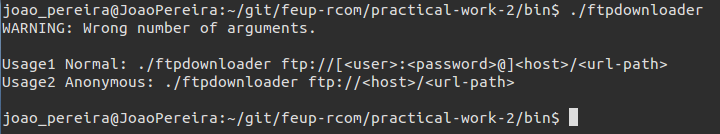
\includegraphics[scale=0.5]{res/usage.png}
\caption{Application usage.}
\end{figure}

A estrutura URL é responsável pelo processamento do argumento especificado na linha de comandos. Esta estrutura contém diversas \textit{strings} que são preenchidas com os diferentes dados presentes no link: \textit{user}, \textit{password}, \textit{hostname}, \textit{path} e \textit{filename}. Após o processamento do URL, o atributo \textit{ip} é preenchido. O atributo \textit{port} é sempre 21 (número da porta de controlo do protocolo FTP).

\begin{figure}[h!]
\centering
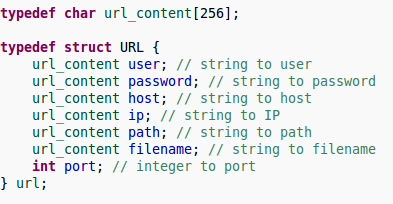
\includegraphics[scale=0.5]{res/url-struct.png}
\caption{URL struct.}
\end{figure}

As funções características desta camada são apresentadas de seguida.
\pagebreak

\begin{figure}[h!]
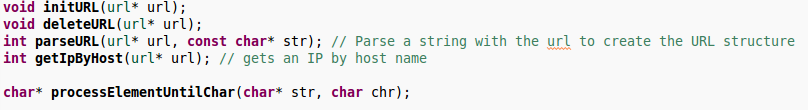
\includegraphics[scale=0.5]{res/url-functions.png}
\caption{URL functions.}
\end{figure}

Breve descrição das funções que constituem esta estrutura:

- \textbf{initURL}, instancia o objecto e aloca memória para os seus atributos;

- \textbf{deleteURL}, liberta a memória alocada anteriormente;

- \textbf{parseURL}, processa o \textit{link} enviado como argumento ao programa e guarda a informação nos respectivos atributos de \textit{url};

- \textbf{getIpByHost}, obtém o IP a partir de um hostname passado como argumento. Este processo deve-se à função \textit{gethostbyname} que retorna uma estrutura do tipo \textit{hostent}, que é usada na função \textit{inet\_ntoa} através de um cast para uma estrutura do tipo \textit{in\_addr} e é devolvido um \textit{char$*$} no formato de números e pontos representando o IP.

A função \textbf{processElementUntilChar} processa uma sub-string até um determinado caracter passado como argumento.\linebreak

No que diz respeito à estrutura do cliente FTP, apenas são necessários dois atributos: um descritor de ficheiro para o controlo e outro para os dados.

\begin{figure}[h!]
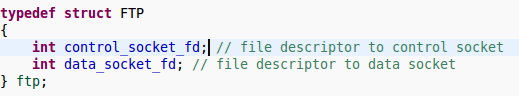
\includegraphics[scale=0.5]{res/ftp-struct.png}
\caption{FTP Client struct.}
\end{figure}

Após o processamento do \textit{URL} estar concluído, é necessário ligar o cliente FTP através de um socket TCP ao servidor em questão, neste caso FTP. Para isso utiliza-se a função \textbf{ftpConnect}. Com uma ligação realizada com sucesso foi preciso ter cuidado com a ordem correcta dos comandos a passar ao servidor para iniciar a transferência do ficheiro. Seguindo o protocolo FTP e a primeira aula laboratorial o grupo estabeleceu uma ordem de comandos a enviar que será analisada na apresentação de resultados desta parte. A ordem pela qual a comunicação foi feita foi:

 -\textbf{USER user}, em que é enviado o nome do utilizador;
 
 -\textbf{PASS pass}, onde o utilizador envia a password para o servidor;
 
 -\textbf{CWD path}, permite ao servidor alterar o directório em que se encontra indo para o correcto onde se encontra o ficheiro;
 
 -\textbf{PASV}, entrada em modo passivo, permitindo uma mútua comunicação entre o servidor e o cliente FTP. É também feita nova conexão do socket mas desta vez a uma porta processada com informação recebida do servidor, sendo guardada no descritor de dados do cliente FTP;
 
 -\textbf{RETR filename}, onde é pedido ao servidor o envio do ficheiro para download.
 
Ao fim de realizados estes passos a transferência do ficheiro desejado pelo utilizador tem o seu início. As funções utilizadas para estas comunicações entre o cliente FTP e o servidor são as seguintes.

\begin{figure}[h!]
\centering
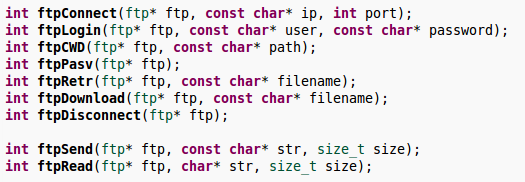
\includegraphics[scale=0.5]{res/ftp-functions.png}
\caption{FTP Client functions.}
\end{figure}

Um ponto importante a frisar na comunicação das duas camadas é que o cliente FTP recorre aos atributos do URL previemente formado para executar todas as acções de comunicação e posterior transferência de ficheiro, não existindo mais nenhuma relação entre ambas.

\subsection{Resultados de download}
TODO

\section{Parte 2 - Configuração da rede e análise}
\subsection{Experiência 1 - Configurar um IP de rede}
A finalidade desta experiência foi a compreensão da configuração de IP’s em máquinas diferentes, de modo a que estas consigam comunicar entre si. Assim, após a configuração dos IP’s das portas eth0 de dois computadores e a adição das rotas necessárias à tabela de reencaminhamento, foi enviado o sinal “ping” de um para o outro para verificar que de facto as máquinas tinham ligação entre si.

Para a configuração dos computadores foi utilizado os comandos $<$ifconfig porta ip$>$ que define o ip da interface para o ip passado como argumento. Após esta configuração executamos um ping de uma máquina para a outra com os ip’s definidos e tivemos sucesso. Foi também possivel ver os pedidos ARP, com os pings definidos e a resposta da maquina correspondente com o seu endereço MAC.

\begin{figure}[h!]
\centering
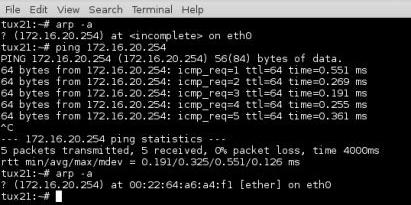
\includegraphics[scale=0.5]{res/image1.jpg}
\end{figure}

O ping após obter o endereço MAC através dos pacotes ARP, gera pacotes do protocolo ICMP. Em frames do tipo Ethernet, os bits vinte e um e vinte e dois do frame identificam o protocolo para o qual deve ser enviado o payload.

\pagebreak

Please see Figure ~\autoref{fig:teste}
A interface loopback é uma interface de rede virtual que o computador utiliza para comunicar com ele próprio, com o objectivo de realizar testes de diagonóstico ou aceder a servidores na própria máquina, como se fosse um cliente. Assim a vantagem de uma interface loopback é que nos permite ter um endereço ip no router que está sempre activo em vez de ser dependente de uma interface física.

\subsection{Experiência 2 - Implementar duas LAN's virtuais no switch}
Nesta experiencia foram criadas 2 Vlans no switch, e adicionadas as maqinas 1 e 4 à primeira Vlan e o máquina 2 a segunda Vlan. Com esta configuração a máquina 2 deixaria de ter acesso ás maquinas 1 e 4 uma vez que se encontram em subredes diferentes.


Para a configuração do switch foi necessário entrar na  sua consola de configuração e executar o comando $<$vlan n$>$ em que n é o numero identificador da vlan. Após a configuração das vlan foi necessário as portas do switch ás respectivas vlans, para criar assim duas subredes individuais. Para tal, usou-se os comandos $<$interface fastethernet 0/i$>$ em que i é o identificador da porta do switch, seguido de $<$switchport mode access$>$ e $<$switchport access vlan n$>$ em que n é o identificador da vlan crianda.

%image3%

Após estas configurações tentamos executar um ping para a máquina 2, o que falhou como era esperado, uma vez que se encontra numa sub rede diferente que não era acessível nem pela máquina 1 nem pela máquina 4.

\subsection{Experiência 3 - Configurar um router em Linux}
O objectivo desta experiência era configurar a máquina 4 como router entre as duas sub redes criadas na experiência dois.

Para realizar esta tarefa foi necessário ligar a interface ethernet 1 da máquina 4 e configura-la com um ip dentro da mesma gama que a máquina 2 e adicionar esta interface à sub rede da máquina 2.

Após esta configuração adiciona-se uma rota à máquina 1 utilizando o comando $<$route add –net  172.16.y1.0/24 gw 172.16.y0.254$>$, o primeiro endereço identifica a gama de endereços para a qual se quer adicionar a rota, e o segundo endereço identifica o ip para a qual reencaminhar o pacote, neste caso o ip da máquina 4. Após isto repete-se o mesmo procedimento para a máquina 2, mas utilizando os seguintes endereços $<$route add –net 172.16.y0.0/24 gw 172.16.y1.253$>$, mais uma vez o ip 172.16.y1.253 é o ip da máquina 4 nesta sub rede.

Depois destas configurações foi possível pingar a máquina 2 a partir da máquina 1, o pedido para o ip da máquina 2 (172.16.y1.1) é reencaminhado para a máquina 4 (172.16.y0.254), como a máquina 4, está ligada à sub-rede de ambas as máquinas, consegue aceder a máquina 2 (172.16.y1.1) através da sua interface eth1 que está nessa sub-rede e assim reencaminha o pacote para a máquina 2. Na resposta o processo é idêntico, sendo o pacote reencaminhado da máquina 2, para a máquina 1.



\subsection{Experiência 4 - Configurar um router comercial e implementar o NAT}
Nesta experiência pretendia-se que fosse configurado um router comercial com nat devidamente implementado. A implementação do nat (Network Adress Translation), teve como objectivo dar a possibilidade dos computadores da nossa rede privada comunicarem com redes externas à nossa. Por se tratar de uma rede privada, os nossos ip’s nunca seriam reconhecidos fora da nossa rede. Por isso criou-se uma técnica que permite rescrever os ip’s de origem  de uma rede interna, para que possam aceder a uma rede externa. Este procedimento gera um número de 16 bits, utilizando esse valor num hash table e escreve-o no campo da porta de origem. Na resposta o processo é revertido e o router sabe para que computador da rede interna deve enviar a resposta.

Para configurar o router é necessário inicialmente configurar a interface interna no processo de nat. Para isso,entra-se na consola de configuração da interface fastethernet 0/0 do router, com o comando $<$interface fastethernet 0/0$>$, além disso tem de ser especificado qual o ip para essa interface, introduzindo o comando $<$ ip address ip mask $>$ que no nosso caso, o ip correspondeu ao 172.16.21.254 e o mask 255.255.255.0.  Após isto é necessário configurar a interface externa, atribuindo um ip à interface 1, que está ligada ao router da sala. Para isso introduz-se os seguintes comandos : $<$interface fastethernet 0/1$>$, $<$ip adress 172.16.1.29 255.255.255.0$>$. Para ambos os casos é necessário que seja introduzido o comando $<$no shutdown$>$, para que estas configurações se mantenham caso o router seja desligado. De seguida, é necessário que seja garantido a gama de endereços introduzindo os comandos $<$ip nat pool ovrld 172.16.1.29 172.16.1.29 prefix 24$>$ e $<$ip nat inside source list 1 pool ovrld overload$>$. Deve ainda ser criada uma lista de acessos e permissoes de pacotes, para cada uma das sub redes, com o comando $<$acesslist 1 permit ip máximo$>$ no nosso caso o ip foi 172.16.20.0 e 172.16.21.0 que poderia ir até 172.16.2X.255, colocando 0.0.0.255 no campo máximo.
Finalmente foram definidas as rotas internas e externas, aplicando $<$ip route 0.0.0.0
0.0.0.0 172.16.1.254$>$ e $<$ip route 172.16.20.0 255.255.255.0 172.16.21.253$>$, este comando cria uma rota, quando o ip de destino for 172.16.20.0-255 deve redireccionar os pacotes para o ip 172.16.21.253.
Para testar, executamos na máquina 1 um ping ao router da sala e verificamos que os pacotes enviados para a máquina 1, passam pela máquina 2, onde são reencaminhados para o router no ip 172.16.21.254.

\subsection{Experiência 5 - DNS}
O objectivo desta experiência era conseguir aceder a redes externas, conseguindo desta forma aceder à Internet através da nossa rede interna, para isto foi necessário configurar o DNS. 

Esta configuração passa por, em todos os hosts da nossa rede aceder e editar o ficheiro resolv.conf. Este ficheiro é lido cada vez que são invocadas rotinas que providenciam acesso à Internet. No nosso caso editamos o ficheiro colocando “nameserver 172.16.1.1”, que se trata do endereço de ip do servidor a qual deve ser acedido.	

%image 4%

Para testar esta experiência, fizemos o teste de ping usando o “www.google.com”, nos logs verificamos que o DNS pergunta a informação contida num dado domain name, onde este responde com o tempo de vida e o tamanho do pacote de dados.\linebreak
Exemplo:

Query-$>$ www.google.com: Type A, class IN.

Answer-$>$ Name: www.google.com, Type: A, Class: IN, Time to live: 39.

seconds, Data Length: 4, Addr: 173.194.41.206

\subsection{Experiência 6 - Ligações TCP}
Por fim, na experiência 6, tentamos compilar e executar a aplicação desenvolvida e descrita na primeira parte do relatório.
	Para testar a aplicação, acedemos a um servidor ftp e fizemos download de um ficheiro. O download efectuou-se correctamente, o que demonstrou que a rede estava bem configurada, não trazendo qualquer problema no acesso por protocolo ftp, assim como à utilização de um servidor exterior à rede.

	TCP utiliza “Selective Repeat ARQ” que é semelhante ao “GO-BACK-N ARQ” com a diferença que o receptor não deixa de processar os frames recebidos quando detecta um erro. Quando existe a detecção da falha de um frame, o receptor continua um “acknowledgement” com o número da frame que falhou. O receptor continua a receber e a processar as frames seguintes, enviando sempre no “ack” o número da frame que falhou primeiro. No final do envio, o emissor verifica os “ack “ e reenvia os frame perdidos.

\section{Conclusões}
Após a realização deste trabalho concluímos com sucesso os principais objectivos do projecto, configurar uma rede e eleborar uma aplicação de download que fosse capaz de executar utilizando a rede criada. 

Desta forma, adquirimos competências e conhecimentos importantes de como configurar uma rede de comunicaçãoe além disso, ficamos com um conhecimento mais alargado sobre diferentes tipos de protocolos utilizados para a comunicação e troca de informação numa rede de computadores.
 
Em suma, podemos afirmar que os objetivos a que nos propusemos na elaboração deste trabalho foram atingidos e que sem dúvida a elaboração deste projeto ajudou a assimilar e fortalecer alguns conhecimentos de redes de computadores e de protocolos da ligação utilizados.

\clearpage
\addcontentsline{toc}{section}{Referências}
\renewcommand\refname{Referências}
\bibliographystyle{plain}
\bibliography{myrefs}


\newpage
\appendix
\section{Anexos}

\subsection{Código da aplicação}
Código da aplicação.

\subsection{Comandos de configuração}
Comandos de configuração.

\subsection{Logs gravados}
Logs gravados.

\begin{figure}[h!]
\caption{Experiência 1 - WireShark}
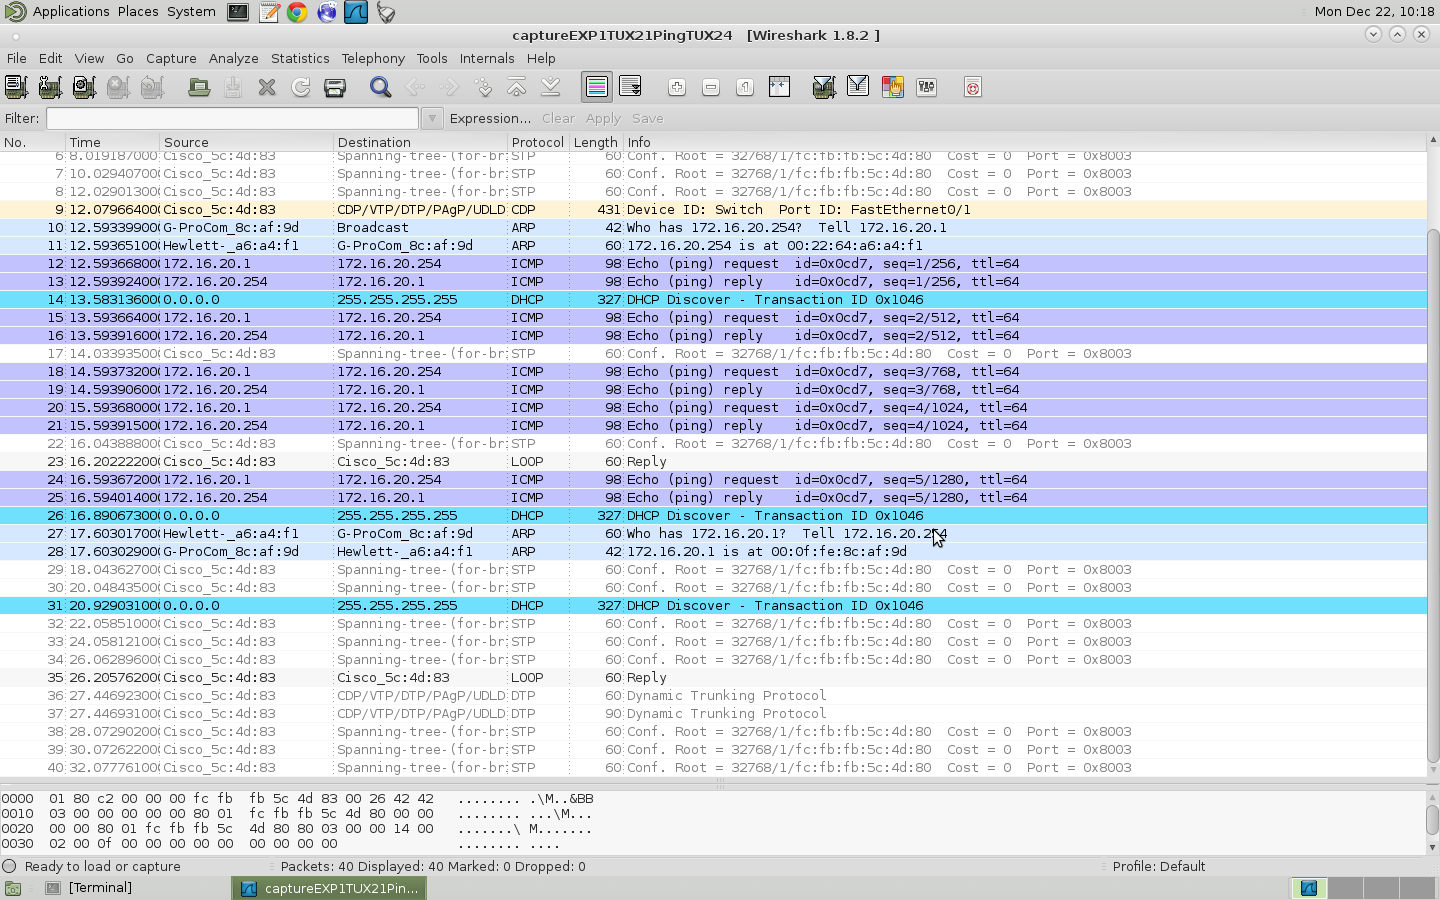
\includegraphics[scale=0.25]{res/image2.png}
\label{fig:teste}
\end{figure}

\end{document}
